\section{Introduction}

JavaScript is one of widely used programming languages not only for client-side
but also for server-side programming~\cite{nodejs, meanjs}
and even small embedded systems~\cite{espruino, tessel2}.
According to W3Techs\footnote{https://w3techs.com/technologies/details/cp-javascript/all/all},
95.2\% of websites use JavaScript as the client-side programming language.
Moreover, JavaScript is the top-ranked language used in active GitHub repositories
\footnote{https://githut.info/}.
Despite its popularity, JavaScript developers often suffer from its intricate semantics
and it may causes security vulnerabilities. For example, the following JavaScript
code seems to always return \( \code{false} \):
\begin{lstlisting}[style=myJSstyle]
function f(x) { return x == !x; }
\end{lstlisting}
Unfortunately, it returns \( \code{true} \) when the argument is an empty array
\( \code{[]} \). To correctly understand such situations, the understanding of
formal semantics of JavaScript is necessary.

\begin{figure}
  \centering
  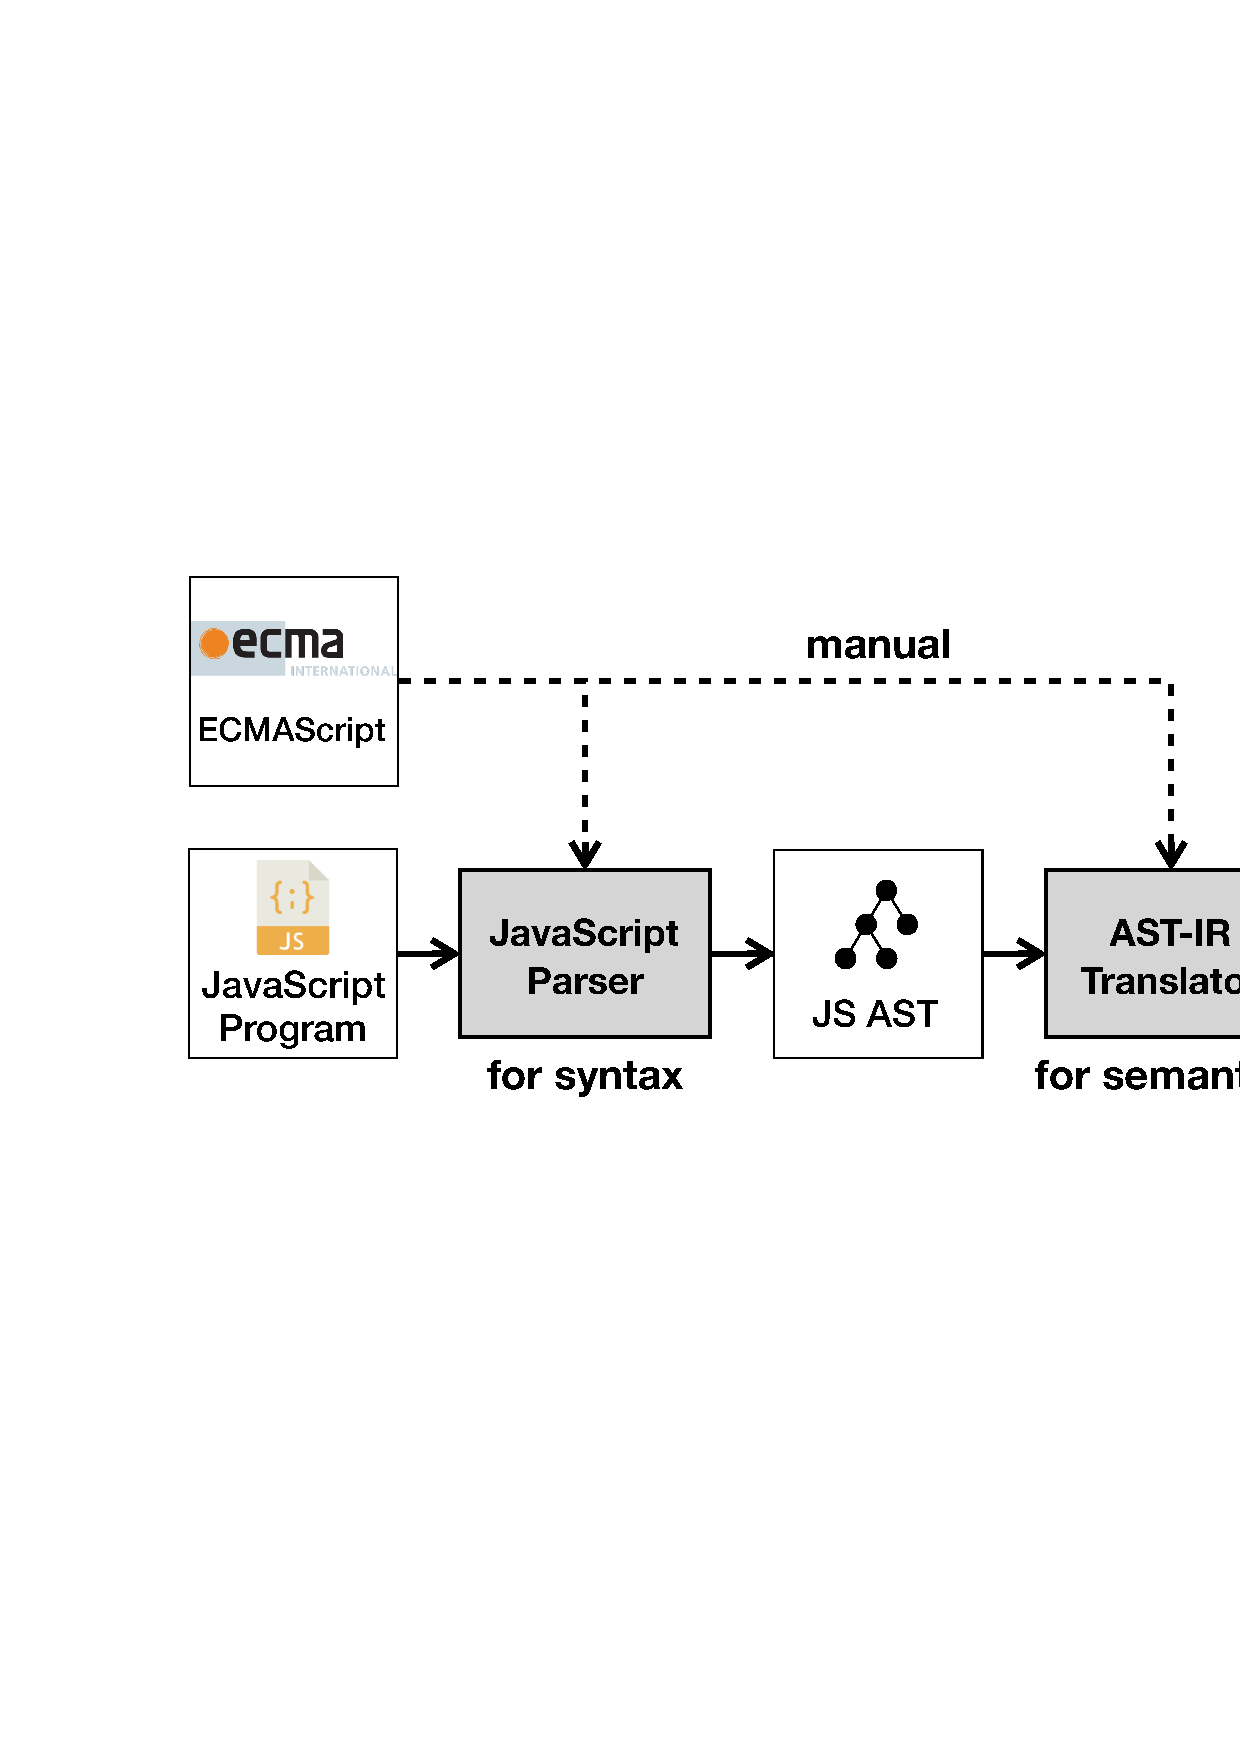
\includegraphics[width=0.48\textwidth]{img/existing.png}
  \caption{Existing approaches of IR-based semantics extractions for ECMAScript}
  \label{fig:existing}
\end{figure}

There have been several researches~\cite{lambdajs, kjs, javert} to define formal semantics of JavaScript
for formal verification or program analysis. As illustrated in Figure~\ref{fig:existing},
they define their own Intermediate Representations (IR) to represent JavaScript
program semantics. They develop a parser for JavaScript programs and
an AST-IR translator to convert JavaScript AST into their own IR.
This approach helps us focus on IR to construct program analysis and formal verifications.
It reduces the effort to handle the diverse and enormous features of JavaScript languages.
We define such methodology that mechanizes to translate given AST into a treatable IR
as \textit{IR-based semantics extractions}.

However, existing IR-based semantics extractions of JavaScript are not easy to
handle recent JavaScript programs because they manually extract semantics.
The JavaScript syntax and semantics are described in ECMAScript specifications.
ECMAScript is a standardized language of JavaScript and written in structured natural languages.
However, the problem is the amount of JavaScript syntax and semantics are huge.
The most recent version of ECMAScript 2019 consists of 798 pages.
Thus, it is excessively labor-intensive to handle full semantics and also error-prone.

Moreover, it is not a suitable approach to cope with the updates of ECMAScript specifications.
Most of formal semantics of ECMAScript supports only ECMAScript 5.1 that was
released in December 2009. Until 2014, it was not a big deal because ECMAScript
specifications are rarely updated. However, in late 2014, The Ecma Technical
Committee 39 (TC39) decided to release ECMAScript on a yearly cadence. From the
ECMAScript 6, officially ECMAScript 2015, they updated specifications every years
in June. Now, no researches correctly deal with recent ECMAScript features;
lexical bindings (\( \code{let} \)), spread operator (\( \code{...} \)),
classes, \( \code{for-of} \) operators, \( \code{async} \) functions, or generators.

In this paper, we propose JavaScript IR-based Semantics Extraction Toolchain (\( \tool \))
based on ECMAScript specifications. The tool automatically extracts JavaScript
syntax and semantics from ECMAScript specifications. It generates JavaScript parser
from the syntax provided by ECMAScript specifications. It also automatically extracts
formal JavaScript semantics with given \textit{compile rules}. Each compile
rule describes how abstract algorithms in specifications are converted into
functions of our intermediate representation \( \ires \) for ECMAScript.
However, to save the labor of defining such rules, we also propose a \textit{rule generation assistant}.
It suggests new compile rules based on statistical analysis of not yet convertible algorithms.
The assistant helps us deal with changed or newly introduced algorithms defined in new versions of
ECMAScript specifications as well.

Our main contribution is our tool \( \tool \) that mechanizes extraction of JavaScript syntax and semantics
from ECMAScript specifications:
\begin{itemize}
  \item \( \tool \) enables to extract the syntax and semantics of ECMAScript 2020,
    which is the next released version of ECMAScript in June 2020.
    Moreover, we successfully applied our tool into the next proposed version,
    ECMAScript 2020. The official conformance test suite, test262, provides
    \inred{XXXXX} tests for ECMAScript 2020 and we passed \inred{XXXXX} tests
    among them.
  \item \( \tool \) is also applicable in-process proposed language features in a modular way.
    ECMAScript specifications are open-source based documentations. Thus, anyone
    could propose some new language features. Then, the committee carefully inspects
    such proposals and adds them into specifications. Each in-process proposed language
    feature has its own specification and tests. Thus, we apply \( \tool \) into the specification
    and evaluate the corresponding tests. Among \inred{XX} proposals, we successfully
    pass all the tests in \inred{XX} proposals and partially pass the tests in \inred{XX}
    proposals.
  \item Moreover, all extraction mechanisms in \( \tool \) is automatic thus we could use this tool
    to find possible specification errors. We found \inred{X} possible specification errors
    in ECMAScript 2020 and reported them into TC39, which is the Ecma Technical Committee.
    We confirm that all of them are real specification errors.
\end{itemize}
